\section{Kognitiv distribusjon og kapasitet}
\label{chp: kognisjon}

Ofte vil arbeidsaktiviteter bestå av flere sammenflettede oppgaver i en gitt tidsramme. Jo lenger tid det tar å utføre en oppgave, jo større sjanse er det for at andre oppgaver eller handlinger må utføres i løpet av denne perioden. Disse oppgavene kan ha ulik avbruddsverdi - prioritet, personlig- eller sosial viktighet, hastegrad ol. \cite{Rogers94}. 
Ved frembruddet av CSCW mot slutten av 80-tallet, oppsto utfordringene om hvordan datasystemer bør designes for å støtte grupper av individer som kommuniserer og arbeider sammen \cite{Rogers94}. 

\tikzstyle{mybox} = [draw=black, fill=white, very thick,
    rectangle, inner sep=10pt, inner ysep=20pt, rounded corners]
\tikzstyle{fancytitle} =[fill=black, text=white]
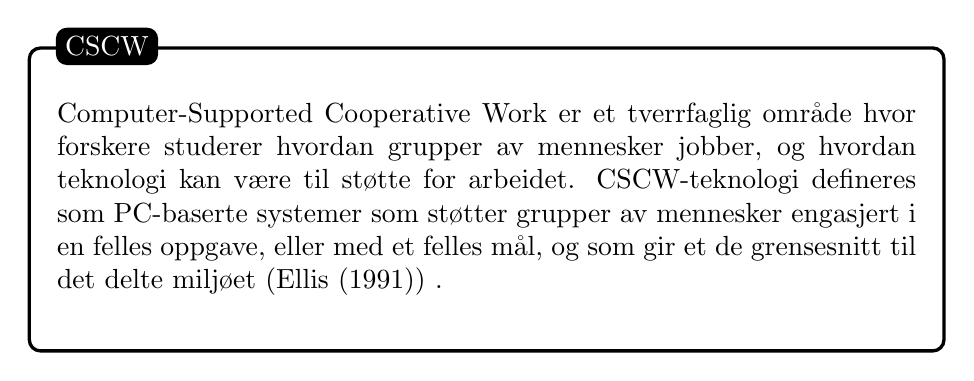
\begin{tikzpicture}
\node [mybox] (box){%
    \begin{minipage}{0.9\textwidth}
     Computer-Supported Cooperative Work er et tverrfaglig område hvor forskere studerer hvordan grupper av mennesker jobber, og hvordan teknologi kan være til støtte for arbeidet. CSCW-teknologi defineres som PC-baserte systemer som støtter grupper av mennesker engasjert i en felles oppgave, eller med et felles mål, og som gir et de grensesnitt til det delte miljøet (Ellis (1991)) \nocite{Ellis91}.
    \end{minipage}
};
\node[fancytitle, rounded corners, right=10pt] at (box.north west) {CSCW};
\end{tikzpicture}%


\noindent
Gitt at mange arbeidsaktiviteter er kognitive, de krever tenkning, problemløsing og evne til å forutse og ta beslutninger, argumenterer Rogers (1994) for at det kreves en forståelse for hvordan disse aktivitetene utføres for å kunne designe datasystemer som kan støtte både kognitive aktiviteter og sosial interaksjon.

\tikzstyle{mybox} = [draw=black, fill=white, very thick,
    rectangle, inner sep=10pt, inner ysep=20pt, rounded corners]
\tikzstyle{fancytitle} =[fill=black, text=white]
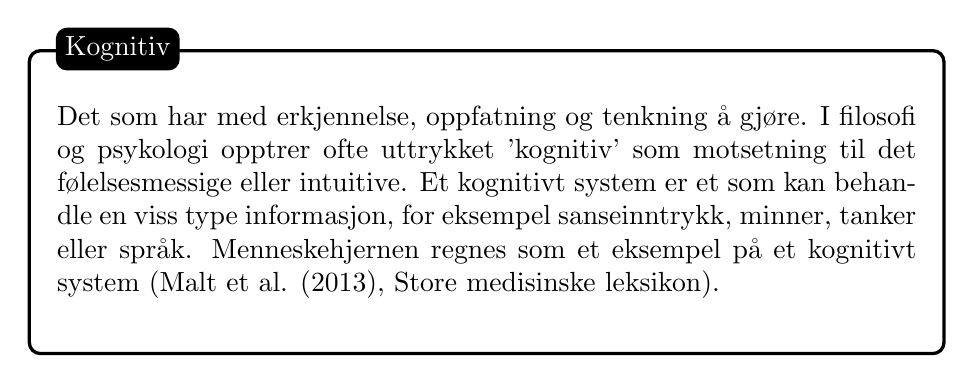
\begin{tikzpicture}
\node [mybox] (box){%
    \begin{minipage}{0.9\textwidth}
     Det som har med erkjennelse, oppfatning og tenkning å gjøre. I filosofi og psykologi opptrer ofte uttrykket 'kognitiv' som motsetning til det følelsesmessige eller intuitive. Et kognitivt system er et som kan behandle en viss type informasjon, for eksempel sanseinntrykk, minner, tanker eller språk. Menneskehjernen regnes som et eksempel på et kognitivt system (Malt et al. (2013), Store medisinske leksikon).
    \end{minipage}
};
\node[fancytitle, rounded corners, right=10pt] at (box.north west) {Kognitiv};
\end{tikzpicture}%

\subsubsection{Distribuert kognisjon}
Distribuert kognisjon, som presentert av Randell et al. (2010), omhandler hvordan kognisjon er distribuert mellom individer i en gruppe. Nemeth et al. (2004) definerer distribuert kognisjon som den delte bevisstheten av mål, planer og detaljer som ingen enkeltperson alene kan begripe. For å være effektiv må denne bevisstheten og forståelsen være nøyaktig og grundig nok til at man sammen kan nå ønskede mål. Som beskrevet av både Randell (2010) og Nemeth (2004), kan kognitive artefakter være til støtte for samarbeid. Dette kan være gjenstander som timeplaner, lister og skjermer. Disse kan være private ved at de gir informasjon til en enkelt bruker, eller de kan være offentlige og distribuere informasjon, for å opprettholde oversikt over det totale arbeidet.

\subsubsection{Kognitiv kapasitet}
“Stacking” defineres av Ebright (2010) som den usynlige beslutningsprosessen sykepleiere utfører om hva, hvordan og når de skal gi pleie til en tildelt gruppe pasienter. Stadige endringer i omgivelsene og informasjonsflyt resulterer i en kontinuerlig re-prioritisering av hvilke oppgaver man skal gjøre når. Dette kombinert med avbrytelser fra omgivelsene, kan resultere i en kognitiv belastning som kan hemme oppmerksomheten. Parker og Coiera (2000) hevder at en begrensende faktor i enhver kommunikasjonsanalyse er den kognitive kapasiteten individer har til å gjennomføre sitt arbeid, da studier har vist at feil og ineffektivitet er et resultat av at denne kapasiteten overskrides. Kunnskap om menneskets hukommelse hevdes å være nøkkelen til å forstå hvilke krav som bør settes til teknologi brukt i slike omgivelser. Det skilles normalt mellom langtids- og korttidsminne. Den passive kunnskapen man besitter ligger i langtidsminnet, for eksempel medisinske fakta eller viktige datoer, mens kortidsminnet, eller arbeidsminnet, er den bevisste delen av minnet som aktivt behandler informasjon. Arbeidsminnet har begrenset kapasitet og varighet, og lar seg raskt forstyrre av distraksjoner og avbrytelser. Coiera og Tombs (1998) \nocite{Coiera98} antyder at synkron kommunikasjon, ansikt-til-ansikt eller per telefon, foretrekkes fordi det gir en umiddelbar bekreftelse på at en beskjed er mottatt. Dersom man ønsker å gi en beskjed eller et ansvar videre, vil usikkerheten om beskjeden er mottatt bli liggende i arbeidsminnet frem til man får en bekreftelse fra mottaker. 



